\subsubsection{Sample Dimensions}
\noindent Three timber lap joint  sample were tested on 26 February 2026 using the Machine at ITC lab. The samples are the stepped lap joint geometry. The shear plane area $A$ is defined as the width $b$ multiplied by the shear height $h^{\prime}$.

\begin{table}[H]
\centering
\begin{tabular}{CCCCCCCCC}
\hline
No. & $a (mm)$ & $b (mm)$ \\ \hline
1  & &  \\
2  & & \\
3  & &  \\\hline
\end{tabular}
\end{table}
\begin{figure}[H]
\centering
\begin{minipage}{0.45\textwidth}
\centering
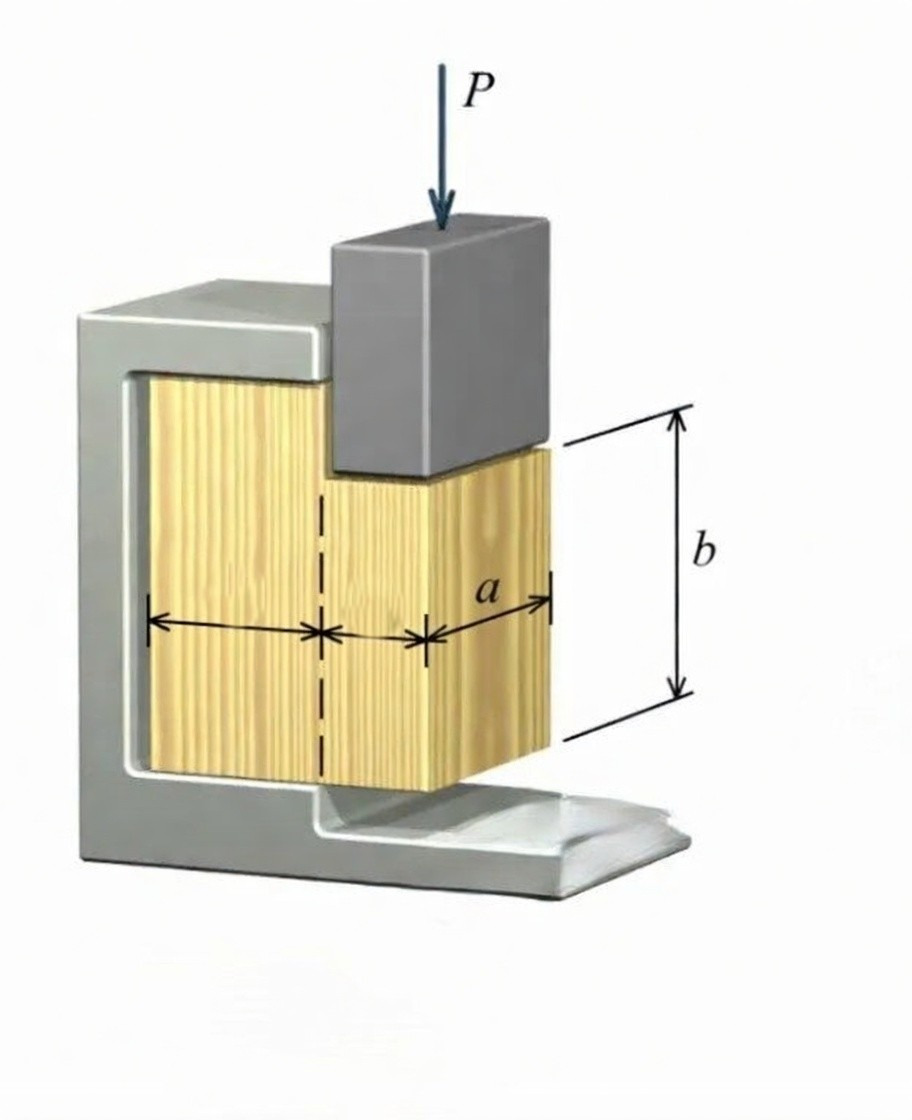
\includegraphics[width=\linewidth]{sample4/image/sampledimension.jpg}
\end{minipage}
\begin{minipage}{0.45\textwidth}
\centering
\includegraphics[width=\linewidth,angle=-90]{sample4/image/sheartestsample.JPG}
\end{minipage}
\caption{Shear testing's sample}
\end{figure}
